\chapter{Kernel-Based Nonlinear Spatial Transformation}\label{ch:spheremapping}
\section{Introduction}

As proposed in last chapter, objective of the system is to predict subsequent abnormalities by quantifying the deviation of sample. Whereas the original cluster topology in feature space $\Omega^d$ depends on the feature extraction stage $g()$ and may lead to poor performance or even failure of predicting. An optimization using spatial transformation is addressed to solve this problem. More specifically, the designed method is able to maximize angles between vectors of normal cluster centroid to each abnormal cluster center centroids. In this chapter, a kernel based nonlinear spatial transformation is proposed to reshape the feature space to a symmetric topology which has the following features:
 \begin{itemize}
     \item Vectors pointing from normal centroid to different abnormal clusters centroids has no overlapping or cross with each other.
     \item Vectors pointing from normal centroid to different abnormal clusters centroids has maximum mutual cosine distance.
     \item The overlapping part of all clusters is minimized.
 \end{itemize}

%However the geometric structure of clusters in the feature space $\Omega$ depends on the feature extraction stage $\g()$. The geometric structure of extracted feature in Table.\ref{table:features} does not meet the standards mentioned above.


\section{Kernel Method}

First, given that clusters do not meet the symmetric features mentioned above, it's assumed in this chapter that new feature space obtained by non-linear reshaping is noted as $\Phi^{d'}$. This reshaping process is included in Personal Classifier stage (as shown in Fig.\ref{fig:flow}) of the ECG classification system as described in chapter 2. The nonlinear mapping projects each sample $\mathbf{x}_k$   onto a new vector $\mathbf{z}_k$ in a higher dimension space, which can be considered as the union of subspace for each type: $\Phi^{d'}=\{\mathcal{N},\mathcal{S},\mathcal{V},\mathcal{F}\}$, where $d'>d$

Kernel method has been widely applied in the machine learning algorithms, among which nonlinear support vector machine (SVM) has been deployed in numerous applications recently\cite{shawe2004kernel}. Nonlinear kernel method is most efficient when there is a nonlinear relationship between input and output variable. This nonlinear relationship assumption is usually true for ECG classification due to the complex feature vectors for ECG analysis. Therefore, it is practical to apply this method in the ECG analysis.


In nonlinear SVM, the algorithm  minimize the expected error $E[L(y,f(x)]$ so as to obtain classification function $f$, where $L$ is the designated loss function, such as square error $(y-f(x))^2$ \cite{scholkopf1999advances}. Based on input space $x_i\in \Omega$ and classifier mapping function $f$, we first define loss function through following formula:

\begin{align}
    \frac{1}{m}\sum_{j\in \mathbb{N}}L(y_j,f(x_j) + \gamma||f||_K^2
\end{align}

where, $||f||_K^2$ is the norm of $f$ on $H_K$. If $H_K$ is the Hilbert space of linear functions, $f=w' x,~w\in\mathbb{R}^d$. Therefore the loss function can be written as:

\begin{align}
    \frac{1}{m}\sum_{j\in \mathbb{N}}L(y_j,w'x_j) + w'w
    \label{eq:kernel}
\end{align}

Positive constant $\gamma$ known as regularization parameter, controls the balance between training error and the complexity (smoothness) of solution. SVM and other machine learning methods deploy kernel method with selected loss function \cite{evgeniou2000regularization}. In general, the solution to Eq.\ref{eq:kernel} is as the following: 

\begin{align}
    f(x)=\sum_{j\in \mathbb{N}}c_j K(x_j,x)
    \label{eq:kernel2}
\end{align}

where $c_j$ is a real number, $K$ is kernel function, such as polynomial function: $K(x,t)=(x't)^r,~x,t\in \mathbb{R}^d$

Hibert space $H_K$ is usually defined base on feature mapping concept, $\Psi:\Phi^d\to \Phi^{d'}$ where $\Phi^{d'}$ is Hilbert space and $<,>_{\Phi}$  represents inner product. Therefore, Eq.\ref{eq:kernel2} can be also written as:

\begin{align}
    f(x) = \sum_{j\in \mathbb{N}}c_j \Psi(x_j,x)
\end{align}

%%%% FROM HERE
For nonlinear kernel function method, the selection of kernel function plays a decisive role. An effective kernel function generally needs to satisfy Mercer theorem \cite{cristianini2000introduction}. This means the matrix defined by function $\Psi(x_j,x)$ is symmetric positive semi-definite. In general, the selection of kernel function depends on all observations in input space. However, in effect, kernel functions with simple expression, such as polynomial kernel function, Gaussian kernel function and exponential kernel function are usually preferred than complicated kernel function for its simplicity and consistency. Polynomial kernel function is usually applied on normalized data for its explicit expression and steady performance. Whereas degree of freedom of polynomial kernel function is comparatively high which leads to a large of parameters. Gaussian kernel function, a very classic robust radial function, has high robustness when the data includes strong noise. Nevertheless, since Gaussian kernel actually projects samples to a infinite dimensional space, it's difficult to visualize projected observations and interpret the result. Moreover its performance is greatly affected by parameter selection.

In this work, the representative polynomial kernel is selected for the purpose of validating the method and explaining the effect of nonlinear kernel method and optimization on the feature space reshaping. The kernel functions can be written in the following format:

\begin{align}
\mathbf{z}_k
=\mathbf{\Psi_{w}} (\mathbf{x}_k) = 
\begin{bmatrix}
w_{1}  \\
w_{2}   \\
\vdots \\
w_{d^\prime} 
\end{bmatrix}
\circ
\begin{bmatrix}
\psi_1(\mathbf{x}_k)\\
\psi_2(\mathbf{x}_k)\\
\vdots\\
\psi_{d^\prime}(\mathbf{x}_k)
\end{bmatrix}
\label{eq:z}
\end{align}

The example above shows that regardless the selection of kernel function, parameter optimization will play a critical role. For instance, in this work, the process of spatial topology optimization is accomplished by adjusting the coefficients of fixed polynomial basis functions $\psi()$. Since the number of parameters to adjust is very large when the order of polynomial functions is high, exhaustive algorithms are not practical for parameter optimization. Therefore, it's necessary to implement a heuristic optimization algorithm, in which parameters are obtained by maximizing or minimizing a loss function. More specifically, the nonlinear reshaping in this work aims to adjust mapping coefficient  $\mathbf{w} = [w_1,w_2,\dots w_d]^T$ to achieve the ideal symmetry of clusters in the reshaped feature space while maintaining the distance between clusters.


\section{Multiobjective Optimization}

\subsection{Objective Functions}

To illustrate the optimization problem, if we assume the original feature space is the 2-dimension space $\Omega^2$, then the mapping kernel function may adopt second-order polynomial function as follows:

\begin{align}
\nonumber
&\mathbf{x}=[x_1~ x_2]^T,~~ \mathbf{w}=[w_1~ w_2~ \dots~ w_5]^T,~~d=2, ~~d^\prime=5\\
&\psi_1(\mathbf{x})=x_1, \psi_2(\mathbf{x})=x_2, \psi_3(\mathbf{x})=x_1^2, \psi_4(\mathbf{x})=x_2^2, \psi_5(\mathbf{x})=x_1x_2
\label{eq5}
\end{align}

Similar to the loss function in the standard nonlinear kernel method, the following objective functions can be used to represent the symmetrical structure to be obtained:

\begin{align}
\label{eq:obj}
&o_1(\mathbf{w}) = \frac{1}{\underset{c,d=2,\dots,p \text{ and } c\neq d }{\min}\{d(\mathbf{v}_{\mathcal{X}_c},\mathbf{v}_{\mathcal{X}_d})\}} \\ %|a,b=1,2\dots k;a\neq b)
\nonumber 
&o_2(\mathbf{w}) = \frac{SW}{SB}=\frac{\sum_{c=1}^{C}  \sum_{\mathbf{z} \in \mathcal{X}_c}   (\mathbf{z}-\mathbf{c}_{\mathcal{X}_c})^T(\mathbf{z}-\mathbf{c}_{\mathcal{X}_c})}{\sum_{c=1}^{C}\sum_{d=1, d\neq c}^{C}  (\mathbf{c}_{\mathcal{X}_c}-\mathbf{c}_{\mathcal{X}_d})^T(\mathbf{c}_{\mathcal{X}_c}-\mathbf{c}_{\mathcal{X}_d}) }
\end{align}

The maximization of pair cosine distance between vectors $\mathbf{v}_{\mathcal{X}_c}$ connecting the centroid of the normal class to the abnormal classes $\mathcal{X}_c$ can be gained by minimizing $o_1(\mathbf{w})$. In the formula, vectors used to measure symmetry is defined by abnormal sample sets in training set DS1 and the personal normal cluster as follows:

\begin{align}
\mathbf{v}_{\mathcal{X}_i} = \mathbf{c}^k_N -  \mathbf{c}_{\mathcal{X}_i}
\end{align}

On the other hand, $o_2(\mathbf{w})$ represents the ratio of within cluster variance to between-cluster variance, hence controls the separation between clusters. Cosine distance is defined by Eq.\ref{eq:cosine} and these objective functions are deduced from discrimination function of personal classifier in Eq.\ref{eq:personal_discrim}. By minimizing these two objective functions at the same time, the algorithm eliminates the ambiguity while applying cosine distance and hence improve the predicting capacity.

\subsection{Multiobjective Particle Swarm Optimization}

It should be noted that $o_1(\mathbf{w}) $ and $o_2(\mathbf{w})$ are not necessarily independent to each other. Thus the optimization problem here means the jointly minimizing of $o_1(\mathbf{w}) $ and $o_2(\mathbf{w})$ subject to constraint condition $|w|_2=1$. Since this is a non-convex multiobjective optimization problem, closed form solution or optimization methods for convex function are not suitable for this problems. Therefore, this paper adopts multiobjective particle swarm optimization (MOPSO) algorithm to solve it.

Particle Swarm Optimization (PSO) has the advantage of fast-converging, heuristic searching and easy implementation\cite{coello2002mopso, alvarez2005mopso}. Therefore, researchers have already started investigating in extending PSO to multiobjective optimization problems. In the framework of MOPSO, the goal is to solve the typical Pareto optimization problem with the structure of PSO. In other word, it aims at solving optimization problem with two or more conflicting objective functions by approximating the Pareto front. 

%\subsubsection{Pareto Front}

Among all MOPSO algorithms in literature, the algorithm proposed by Coello Coello and Lechug facilitates the implementation and improved the performance compared to other methods\cite{coello2002mopso}. Therefore,  this algorithm is adopted in this work. One featured design of this algorithm is the external repository in which all Pareto optimized particles in each swarm is recorded for each iteration. The configuration of repository members are stored and used as an optimal approximation of the Pareto front of the problem as they converge to the actual Pareto front as proved in \cite{coello2002mopso}. Fig.\ref{fig:repo_members} generated by optimizing $o_1(\mathbf{w}) $ and $o_2(\mathbf{w})$ demonstrates the repository members are Pareto optimal than other particles in the objective function space and they converge to the Pareto front.

\begin{figure}[t]
\centering
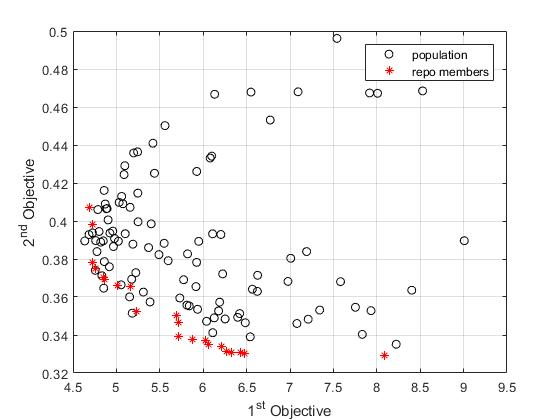
\includegraphics[scale=.6]{Fig/repo_members.jpg}
\caption{Particles stored in external repository approximate the Pareto front}
\label{fig:repo_members}
\end{figure}

With the concept of Pareto front,we further demonstrate the impact of applying kernel functions in this multiobjective optimization problem by comparing Pareto front before transformation with kernel method and the Pareto front with nonlinear reshaping. %A two-dimension curve formed by repository members t will be drawn with two objective functions.

%This mapping by kernel method can be accounted as the input space reshaping, namely, new input sample space is produced using non-linear kernel bending feature space in order for a higher space symmetry. Reshaping result as indicated in diagram 4-6 can be obtained through testing the reshaping algorithm with test data and quadratic polynomial. More specifically, we can regard this kernel method as a mapping from two-dimension space   to three-dimension space. Because the data visualization is very important in the test, we don’t adopt polynomial kernel of higher degree.

As shown in Fig.\ref{fig:pareto_compare}, the Pareto front in feature space after nonlinear reshaping is superior obviously to that of Pareto front with linear combination of original data. The kernel function used in this comparison is a third-order polynomial kernel function as formulated in Eq.\ref{eq5}. The result shows that nonlinear kernel method possess a higher degree of freedom to in multiobjective optimization. In other words, kernel method combined with multiobjective particle swarm optimization algorithm can improve the spatial topology of clusters.

%\subsubsection{Pareto Front}
\begin{figure}[t]
\centering
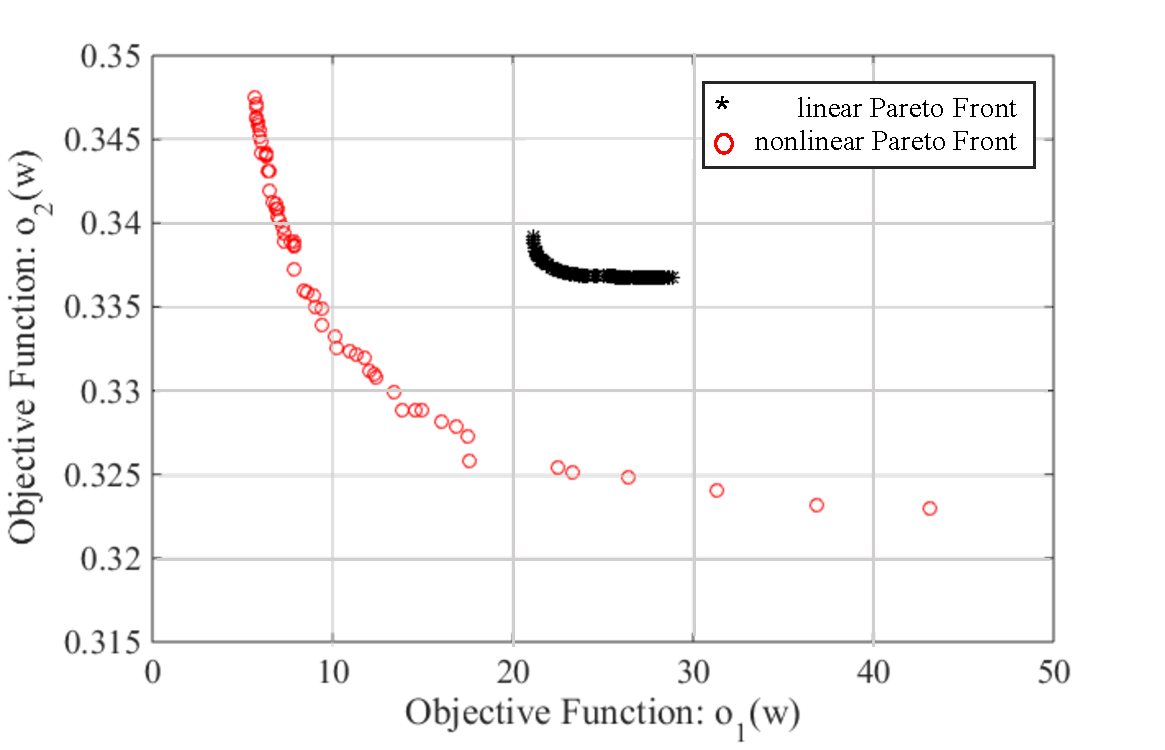
\includegraphics[scale=.6]{Fig/pareto_compare.pdf}
\caption{Increase of degree of freedom in optimization is proved by comparing the Pareto fronts generated by linear and nonlinear basis function}
\label{fig:pareto_compare}
\end{figure}

\section{Experimental Results}

This section will introduce the experimental result generated with test set DS2 of MITDB to show the performance of the proposed method in this Chapter. Here, we firstly map the original 22-dimensional feature vectors representative of cardiac segments into a 8-dimensional vectors $\mathbf{x}_{8 \times 1}$ using principal component analysis (PCA). 
In order to realize the non-linear transformation in (\ref{eq:z}), we use polynomial function of order $3$. Taking the computational cost into account and also to avoid over-fitting of higher-order data samples, we only retain $32$ terms (8 second order pure terms $x_i^2$, 8 third order pure terms $x_i^3$, 8 second order cross terms $x_ix_j$, and 8 pure third order cross terms $x_i x_j^2$) and randomly discard the rest of cross terms. Therefore, the mapped vectors $\mathbf{z}_{32 \times 1}$ include a total of $32$ terms as follows.

\begin{align}
\label{eq:8-32}
\mathbf{z}&=\{x_i^2|i=1,2\dots 8\}\cup\{x_i^3|i=1,2\dots 8\} \cup\\
\nonumber
& \{x_ix_j|i,j=1,2\dots 8,i\neq j\} \cup  \{  x_i^2x_j | i,j=1,2\dots 8,i\neq j \}
\end{align}

The performance of the proposed system in this paper is tested with DS2 excluding record 232, for this record has only 7 normal samples $y_k=N$. In total, 21 records are tested.

Table \ref{table:result1}, shows the performance of the proposed method in classification of ECG signal segments. In order to average the results over all recordings, we present the median, interquartile range (IQR), mean and standard deviation of accuracy (AC), sensitivity (SE) and specificity (SP). The results are promising and the median of accuracy for all classes are in the range of $88\%-99\%$. Sensitivity and specificity of the proposed method exhibits similar ranges. The mean accuracy is at least $86\%$ excluding class $V$. Therefore, this system is very less likely to miss an important alarm or to report false alarms. 

\begin{table}[thpb]
	\caption{Classification results of the proposed method.}
	\centering
	\begin{tabular}{|c||c||c||c||c|}
		\hline
		Class N & median(\%) & IQR(\%) & mean(\%)& std (\%) \\ 
		\hline 
		AC & 94.8& 19.52 & 86.62 & 18.55\\ 
		\hline 
		SE & 97.21  & 17.36 & 87.47 &19.26 \\ 
		\hline 
		class V & median(\%) & IQR(\%) & mean(\%)& std (\%) \\ 
		\hline 
		AC & 86.11 & 27.54 & 76.41 & 22.81 \\ 
		\hline 
		SP & 99.71 & 11.22 & 90.18 & 18.52 \\ 
		\hline 
		class S & median(\%) & IQR(\%) & mean(\%)& std (\%)\\ 
		\hline 
		AC & 99.28 & 2.24& 98.29&2.57 \\ 
		\hline 
		SP & 99.64& 22.17& 97.56 & 6.06\\ 
		\hline 
		class F & median(\%) & IQR(\%) & mean(\%)& std (\%) \\ 
		\hline 
		AC & 97.91 & 8.2&93.85&7.84\\ 
		\hline 
		SP & 100.00 & 0.03&99.12&3.6\\ 
		\hline 
		\hline
	\end{tabular} 
	\label{table:result1}
\end{table}

More importantly, the predicting ability of the proposed method is worthy of evaluating separately. In order to quantify the conditional probability of observing a red alarm after a preceding yellow alarm of similar type in (\ref{eq:personal_discrim}), we count the number of predicted samples as follows:

\begin{align}
\nonumber 
&P(\hat{y}_{k+i}=X_r|\hat{y}_{k}=X_y)=\frac{\text{\# of $y_{k+i}=X$ after $\hat{y}_k=X_y$}}{\text{\# of true alarms after $\hat{y}_k=X_y$}} \\
&P(\hat{y}_{k+i}=X_r)=\frac{\text{\# of true alarm of type $X$ ($y_{k}=X$)}}{\text{\# of all true alarms}} 
\end{align}

The summary of results for all 21 test records is presented in Table. \ref{table:pred}. The last 4 columns of the Table. \ref{table:pred} show the probability of having a subsequent true abnormality of any type after observing a yellow alarm. %It's compared with the probability of having the same type of abnormality after a secondary abnormality of its own type. 
These results confirm the predictive power of yellow alarms. 
For instance, the absolute probability of observing a segment with abnormal classes $V$, $S$, and $F$ is respectively $\frac{96}{96+29+18}=67\%$, $\frac{29}{96+29+18}=20\%$ and $\frac{18}{96+29+18}=13\%$, based on their relative frequencies. However, these probabilities after observing a yellow alarm of type $Vp$ are respectively $\frac{38}{38+11+2}=75\%$, $\frac{11}{38+11+2}=21\%$ and $\frac{2}{38+11+2}=4\%$. This means that the probability of observing a red alarm of type $V$ is $75\%-67\%=8\%$ higher than its absolute probability. The same trend holds for other yellow alarms as well. The results suggest a more in-depth study of the concept of yellow alarms for heart monitoring.

\begin{table}
	\caption{Predictive power of yellow alarms: A yellow alarm increases the chance of observing a red alarm of the same type.}
	\centering
	\begin{tabular}{|m{3.5em}|| m{1.4em} || m{1.4em} || m{1.4em} ||m{1.4em}|| m{1.4em} || m{1.4em} || m{1.4em} || m{1.4em}|}
		\hline
		& \multicolumn{3}{m{8em}}{Number of next abnormality }& &\multicolumn{3}{m{8em}}{Probability of next abnormality (\%)}  & \\ 
		\hline 
		secondary abnormalities & $V_y$ & $S_y$ & $F_y$ & Total & $V_y$ & $S_y$ & $F_y$ & Total \\ 
		\hline 
		True V & 38 & 23 & 35& 96 & 75 & 75 & 61 & 67 \\ 
		\hline 
		True S & 11 & 10 & 8 & 29 & 21 & 29 & 14& 20 \\ 
		\hline 
		True F & 2 & 2 & 14 & 18 & 4 & 6 & 25 & 13 \\ 
		%		\hline 
		%		Total & 4 & 20 & 0 & 24 & 100 & 100 & 100 & 100\\
		\hline 
	\end{tabular} 
	\label{table:pred}
\end{table}


\section{Conclusions}

This chapter explains the nonlinear reshaping with kernel function and multipurpose particle swarm optimization method. With the kernel method adopted in SVM, we utilize a group of nonlinear kernels to reshape the input feature space and map it to high-dimensional feature space, which meets two conditions, namely, maximum separation between cluster and maximum cosine similarities between abnormal clusters.

In this chapter we adopt multipurpose particle swarm optimization method to optimize parameters of kernel function. Result shows that Pareto front produced by kernel method in the objective function space is apparently optimal to that produced by linear combination of features. The results verify the accuracy of the proposed method with a classification accuracy range of $88\%-99\%$ for different ECG records in publicly available MIT-BIH database.

Above all the proposed methodology demonstrates a potential to add detailed information about sample deviation upon conventional machine learning algorithm. We tested this system with ECG signal and observed promising results, but this method is not bound to this application. 
  